\documentclass[11pt,a4paper]{article}

% Packages
\usepackage[margin=1in]{geometry}
\usepackage{graphicx}
\usepackage{xcolor}
\usepackage{fancyhdr}
\usepackage{titlesec}
\usepackage{listings}
\usepackage{booktabs}
\usepackage{multirow}
\usepackage{array}
\usepackage{enumitem}
\usepackage[hidelinks]{hyperref}
\usepackage{tcolorbox}
\usepackage{pdflscape}

% Xilinx-style colors
\definecolor{xilinxred}{RGB}{230,0,0}
\definecolor{xilinxgray}{RGB}{100,100,100}
\definecolor{codebg}{RGB}{245,245,245}

% Header/Footer
\pagestyle{fancy}
\fancyhf{}
\fancyhead[L]{\textcolor{xilinxred}{\textbf{Kepler-Style SIMT GPU Core}}}
\fancyhead[R]{\textcolor{xilinxgray}{Datasheet v1.0}}
\fancyfoot[C]{\thepage}
\renewcommand{\headrulewidth}{2pt}
\renewcommand{\headrule}{\hbox to\headwidth{\color{xilinxred}\leaders\hrule height \headrulewidth\hfill}}

% Section formatting
\titleformat{\section}
  {\color{xilinxred}\Large\bfseries}
  {\thesection}{1em}{}[\titlerule]

\titleformat{\subsection}
  {\color{xilinxgray}\large\bfseries}
  {\thesubsection}{1em}{}

% Code listings
\lstset{
    backgroundcolor=\color{codebg},
    basicstyle=\ttfamily\small,
    breaklines=true,
    frame=single,
    numbers=left,
    numberstyle=\tiny\color{xilinxgray},
    keywordstyle=\color{blue}\bfseries,
    commentstyle=\color{green!60!black},
    stringstyle=\color{red}
}

% Info boxes
\newtcolorbox{infobox}[1]{
  colback=blue!5!white,
  colframe=blue!75!black,
  fonttitle=\bfseries,
  title=#1
}

\newtcolorbox{warnbox}[1]{
  colback=red!5!white,
  colframe=red!75!black,
  fonttitle=\bfseries,
  title=#1
}

\begin{document}

% Title Page
\begin{titlepage}
    \centering
    \vspace*{2cm}
    
    {\Huge\textcolor{xilinxred}{\textbf{Kepler-Style SIMT GPU Core}}\par}
    \vspace{0.5cm}
    {\Large Architecture Specification \& Datasheet\par}
    \vspace{2cm}
    
    \begin{tcolorbox}[colback=xilinxgray!10,colframe=xilinxred,width=0.8\textwidth]
        \centering
        \textbf{Specification Overview}\\[0.5cm]
        Educational GPGPU Processor\\
        5-Stage Pipelined SIMT Architecture\\
        Dual-Issue Superscalar Execution\\
        Hardware 3D Graphics Orchestration\\
        768 Concurrent Threads (24 Warps × 32 Threads)
    \end{tcolorbox}
    
    \vfill
    
    {\large Document Version: 1.0\par}
    {\large \today\par}
\end{titlepage}

\tableofcontents
\newpage

% ============================================================================
\section{Executive Summary}
% ============================================================================

The \textbf{Kepler-Style SIMT Core} is an educational, behavioral model of a General Purpose GPU (GPGPU) processor. Designed for learning and architectural exploration, it implements a 32-thread Single Instruction, Multiple Threads (SIMT) architecture compliant with modern GPU execution models.

\subsection{Key Features}

\begin{itemize}[leftmargin=*]
    \item \textbf{Architecture}: 5-Stage Pipelined SIMT Core (IF, ID, OC, EX, WB)
    \item \textbf{Parallelism}: 32 Threads per Warp, dual-issue capability (up to 2 instructions/cycle)
    \item \textbf{Multithreading}: Fine-Grained Multithreading (FGMT) with 24 warps (768 threads) and zero-overhead context switching
    \item \textbf{Memory Model}:
    \begin{itemize}
        \item Shared Memory: 16KB On-Chip Scratchpad (32 banks) with bank-conflict replay
        \item Global Memory: Coalesced LSU with \textbf{Multi-Line Split Support}
        \item MSHR: 64-entry out-of-order tracking per warp
    \end{itemize}
    \item \textbf{Synchronization}: Hardware Barrier (BAR) with Epoch consistency
    \item \textbf{Control Flow}: Hardware Divergence Stack (SSY/JOIN) and Function Call Stack (CALL/RET)
    \item \textbf{Graphics}: Hardware-accelerated 3D wireframe rendering with Perspective Projection
\end{itemize}

\subsection{Main Implementation}

The core logic is implemented in \texttt{streaming\_multiprocessor.sv}, which contains the complete 5-stage pipeline, warp scheduler, scoreboard, and execution units.

% ============================================================================
\section{Microarchitecture Specification}
% ============================================================================

\subsection{Pipeline Overview}

The core implements an in-order, dual-issue pipeline with out-of-order memory completion.

\begin{table}[h]
\centering
\begin{tabular}{|l|p{10cm}|}
\hline
\textbf{Stage} & \textbf{Function} \\
\hline
\textbf{IF} & Instruction Fetch - Warp scheduler selects ready warp, fetches 2 consecutive instructions \\
\hline
\textbf{ID} & Instruction Decode \& Issue - Dual-issue logic checks dependencies and structural hazards \\
\hline
\textbf{OC} & Operand Collector - Gathers operands from banked register file, handles conflicts \\
\hline
\textbf{EX} & Execute \& Memory - ALU, FPU, SFU operations; LSU calculates addresses and performs cache access \\
\hline
\textbf{WB} & Writeback - Arbitrates results from ALU, FPU, Memory; clears scoreboard \\
\hline
\end{tabular}
\caption{Pipeline Stage Descriptions}
\end{table}

\begin{figure}[htbp]
    \centering
    \includegraphics[width=0.9\textwidth]{pipeline_diagram.png}
    \caption{High-Level Pipeline Overview}
    \label{fig:pipeline_high}
\end{figure}

\begin{figure}[htbp]
    \centering
    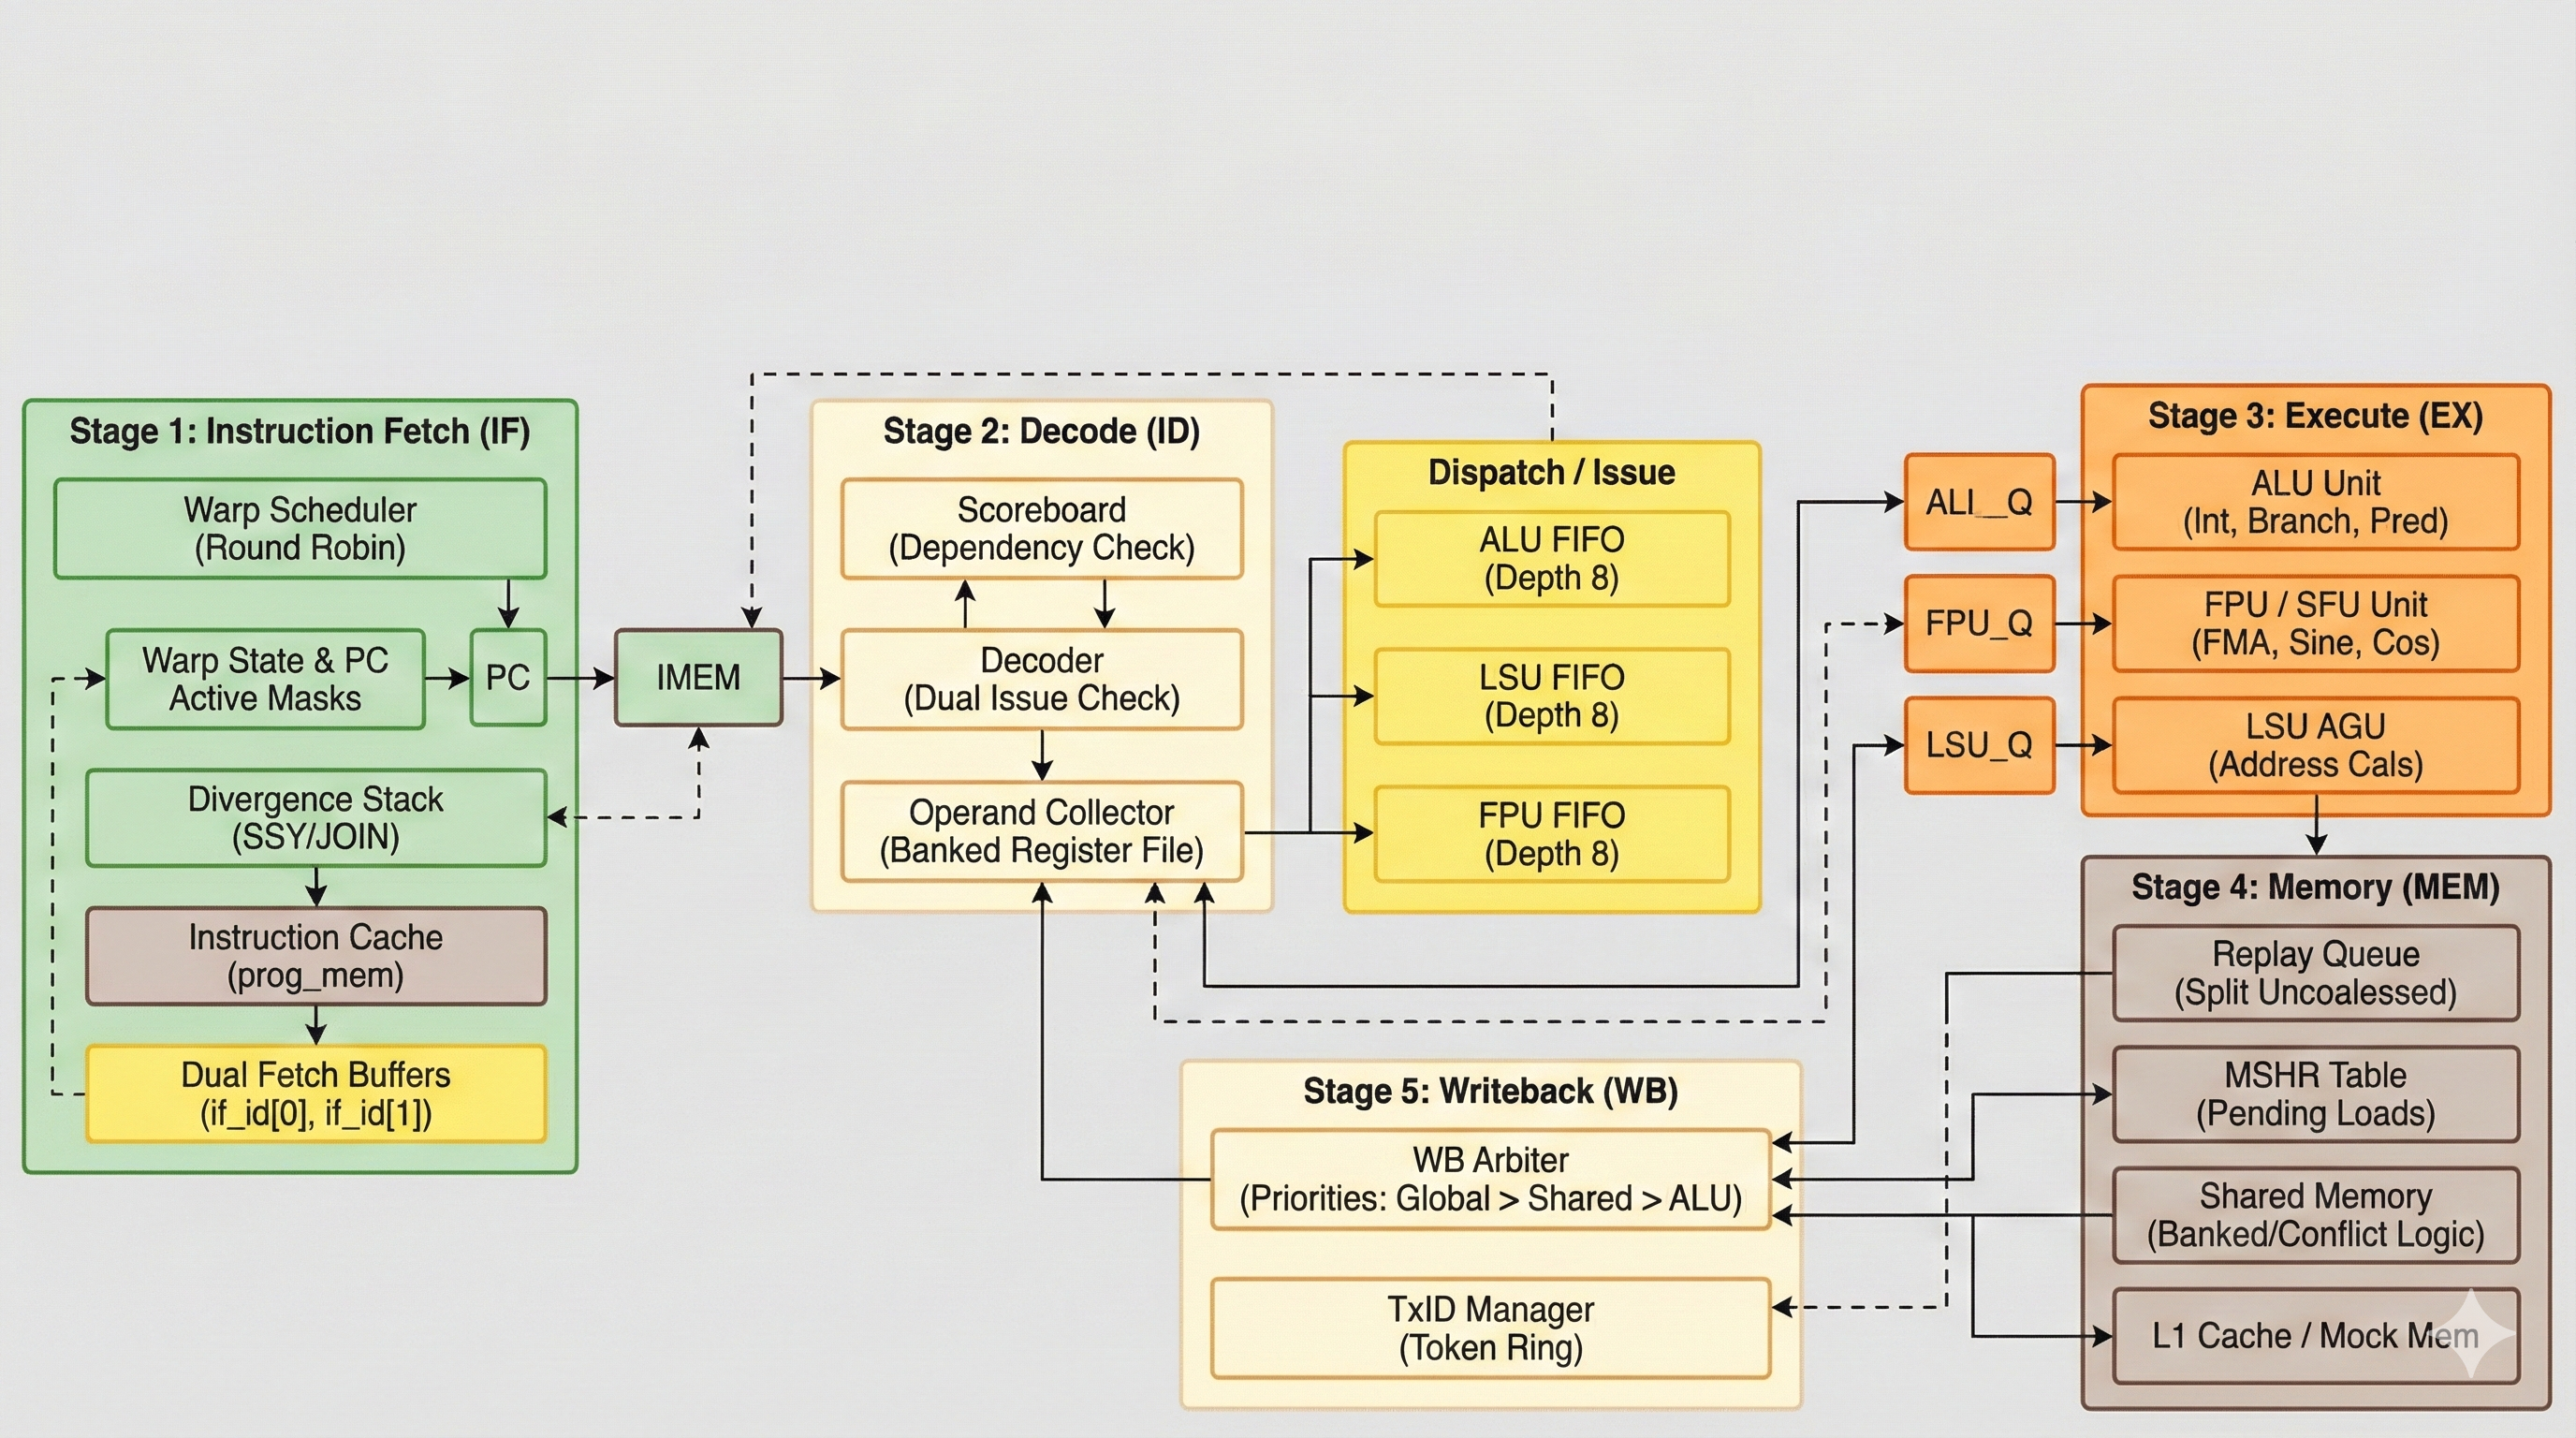
\includegraphics[width=0.9\textwidth]{detailed_pipeline.png}
    \caption{Detailed Dual-Issue SIMT Microarchitecture}
    \label{fig:pipeline_detail}
\end{figure}

\subsection{Thread Hierarchy \& Scheduling}

\begin{infobox}{Warp Organization}
\begin{itemize}[leftmargin=*]
    \item \textbf{32 Threads per Warp}: Executed in lockstep (SIMT)
    \item \textbf{24 Warps per Core}: Supporting up to 768 concurrent threads resident on the SM
    \item \textbf{Warp ID}: 5-bit identifier (0-23)
\end{itemize}
\end{infobox}

\subsubsection{Multithreading Model}

\begin{itemize}[leftmargin=*]
    \item \textbf{Fine-Grained Multithreading (FGMT)}: The core can switch between warps on a cycle-by-cycle basis to hide latency
    \item \textbf{Latency Hiding}: When a warp stalls (scoreboard dependency, memory wait, barrier), the scheduler immediately switches to another ready warp
\end{itemize}

\subsubsection{Scheduling \& Switching Rule}

\begin{itemize}[leftmargin=*]
    \item \textbf{Greedy Scheduling}: The scheduler stays with the same warp as long as it has eligible instructions
    \item \textbf{When do Warps Switch?}:
    \begin{enumerate}
        \item The current warp stalls (RAW dependency, memory operation pending, barrier wait)
        \item The current warp completes (hits EXIT or diverges to inactive state)
    \end{enumerate}
    \item \textbf{Two-Loop Search Mechanism}:
    \begin{itemize}
        \item Outer Loop: Iterates through all 24 warp slots starting from \texttt{rr\_ptr}
        \item Inner Check: Checks eligibility (state = READY, no scoreboard conflicts, OC has space)
        \item First-Match: Selects the first eligible warp found and breaks
        \item Pointer Update: After selection, \texttt{rr\_ptr} advances to \texttt{(selected\_warp + 1) \% 24}
    \end{itemize}
    \item \textbf{Context Switching Overhead}: Zero Cycles - all warp state is hardware-resident
\end{itemize}

\subsection{Dual-Issue Compatibility}

\begin{table}[h]
\centering
\small
\begin{tabular}{|l|l|l|p{5cm}|}
\hline
\textbf{Instruction A} & \textbf{Can Pair With} & \textbf{Cannot Pair With} & \textbf{Reason} \\
\hline
ALU & FPU, LSU, SFU & ALU, CTRL & Same functional unit conflict \\
\hline
FPU & ALU, LSU, SFU & FPU & Same functional unit conflict \\
\hline
LSU & ALU, FPU, SFU & LSU & Only 1 memory port per warp \\
\hline
SFU & ALU, FPU, LSU & SFU & Same functional unit conflict \\
\hline
CTRL & None & All & Control flow must execute alone \\
\hline
\end{tabular}
\caption{Dual-Issue Compatibility Matrix}
\end{table}

\begin{warnbox}{Additional Constraints}
\begin{itemize}[leftmargin=*]
    \item \textbf{RAW Hazard}: Instruction B cannot read a register that A writes
    \item \textbf{WAW Hazard}: Both instructions cannot write to the same destination register
    \item \textbf{Control Flow}: Branches, barriers, synchronization, and function calls always issue alone
\end{itemize}
\end{warnbox}

% ============================================================================
\section{Instruction Set Architecture}
% ============================================================================

\subsection{Instruction Encoding Format (64-bit)}

\begin{verbatim}
+----------+----------+----------+----------+--------+----------------+
|  OPCODE  |    RD    |   RS1    |   RS2    |  PRED  |  RS3 / EXTRA   |
+----------+----------+----------+----------+--------+----------------+
|  8-bits  |  8-bits  |  8-bits  |  8-bits  | 4-bits |     8-bits     |
+----------+----------+----------+----------+--------+----------------+
|                    IMMEDIATE (20-bits)                              |
+---------------------------------------------------------------------+
\end{verbatim}

\begin{itemize}[leftmargin=*]
    \item \textbf{OPCODE}: Specifies the operation (e.g., ADD, LDR, BRA)
    \item \textbf{RD}: Destination Register Index (R0-R63)
    \item \textbf{RS1 / RS2}: Source Register Indices
    \item \textbf{PRED}: Predicate Register Index (P0-P7) and Condition Flags
    \item \textbf{RS3 / EXTRA}: Third Source Register or Branch Target Offset
    \item \textbf{IMMEDIATE}: 20-bit Signed Immediate / Offset
\end{itemize}

\subsection{Opcode Map (Selected Instructions)}

\begin{table}[h]
\centering
\small
\begin{tabular}{|l|l|p{7cm}|}
\hline
\textbf{Opcode} & \textbf{Mnemonic} & \textbf{Description} \\
\hline
\multicolumn{3}{|c|}{\textbf{Integer Arithmetic \& Logic}} \\
\hline
0x00 & NOP & No Operation \\
0x01 & ADD & Integer Addition \\
0x02 & SUB & Integer Subtraction \\
0x03 & MUL & Integer Multiplication \\
0x10 & AND & Bitwise AND \\
0x11 & OR & Bitwise OR \\
0x12 & XOR & Bitwise XOR \\
\hline
\multicolumn{3}{|c|}{\textbf{Memory Operations}} \\
\hline
0x20 & LDR & Load from Global Memory \\
0x21 & STR & Store to Global Memory \\
0x22 & LDS & Load from Shared Memory \\
0x23 & STS & Store to Shared Memory \\
\hline
\multicolumn{3}{|c|}{\textbf{Control Flow}} \\
\hline
0x24 & BRA & Unconditional Branch \\
0x25 & BEQ & Branch if Equal \\
0x26 & BNE & Branch if Not Equal \\
0x27 & CALL & Function Call \\
0x28 & RET & Return from Function \\
0x29 & SSY & Set Synchronization Point \\
0x2A & JOIN & Re-converge Divergent Paths \\
0x2B & BAR & Barrier Synchronization \\
0x2C & EXIT & Terminate Warp Execution \\
\hline
\end{tabular}
\caption{Instruction Set Architecture (Partial)}
\end{table}

% ============================================================================
\section{Subsystem Deep Dive}
% ============================================================================

\subsection{Operand Collector (OC)}

The Operand Collector decouples instruction fetching from operand reading, resolving register file bank conflicts.

\begin{infobox}{Key Mechanism}
\begin{enumerate}[leftmargin=*]
    \item Instructions are allocated to a Collector Unit (CU)
    \item The CU requests operands from the Bank Arbiter
    \item The Arbiter grants access based on bank availability (Bank = RegID \% 4)
    \item Once all operands are collected, the CU dispatches to Execution Units
\end{enumerate}
\end{infobox}

\subsection{Divergence Stack (SSY/JOIN)}

To handle SIMT divergence on control flow, the core maintains a per-warp Divergence Stack.

\textbf{Divergence \& Serialization}:
\begin{enumerate}[leftmargin=*]
    \item Pushes current Active Mask, PC, and Token onto stack via SSY
    \item Updates Active Mask to only enable threads taking the branch
    \item Serializes execution: "then" path executes first, then "else" path
    \item After all paths complete, JOIN pops the stack and restores full Active Mask
\end{enumerate}

\begin{warnbox}{Performance Impact}
Divergent paths are executed \textbf{serially} (one after another), not in parallel, which can reduce effective throughput when warps diverge frequently.
\end{warnbox}

The core implements a robust memory hierarchy with a non-blocking Coalesced Load/Store Unit (LSU).

\textbf{LSU Split Handling}:
The LSU automatically detects when a warp's memory accesses span multiple 128-byte cache lines. It utilizes a hardware-managed \textbf{Replay Queue} to serialize these into multiple sequential requests to the memory system. This process is transparent to the warp scheduler, allowing uncoalesced requests to progress without software intervention.

\begin{table}[h]
\centering
\begin{tabular}{|l|p{10cm}|}
\hline
\textbf{Component} & \textbf{Description} \\
\hline
MSHR Table & 64-entry table per warp tracking pending memory operations \\
\hline
Transaction ID & 16-bit ID: [5:0] Slot ID, [9:6] Warp ID, [15:10] SM ID \\
\hline
FIFO Management & Free IDs managed via per-warp FIFO (pop on issue, push on response) \\
\hline
Scoreboard & Prevents RAW hazards by blocking dependent instructions until response arrives \\
\hline
\end{tabular}
\caption{Memory Subsystem Components}
\end{table}

\begin{figure}[htbp]
    \centering
    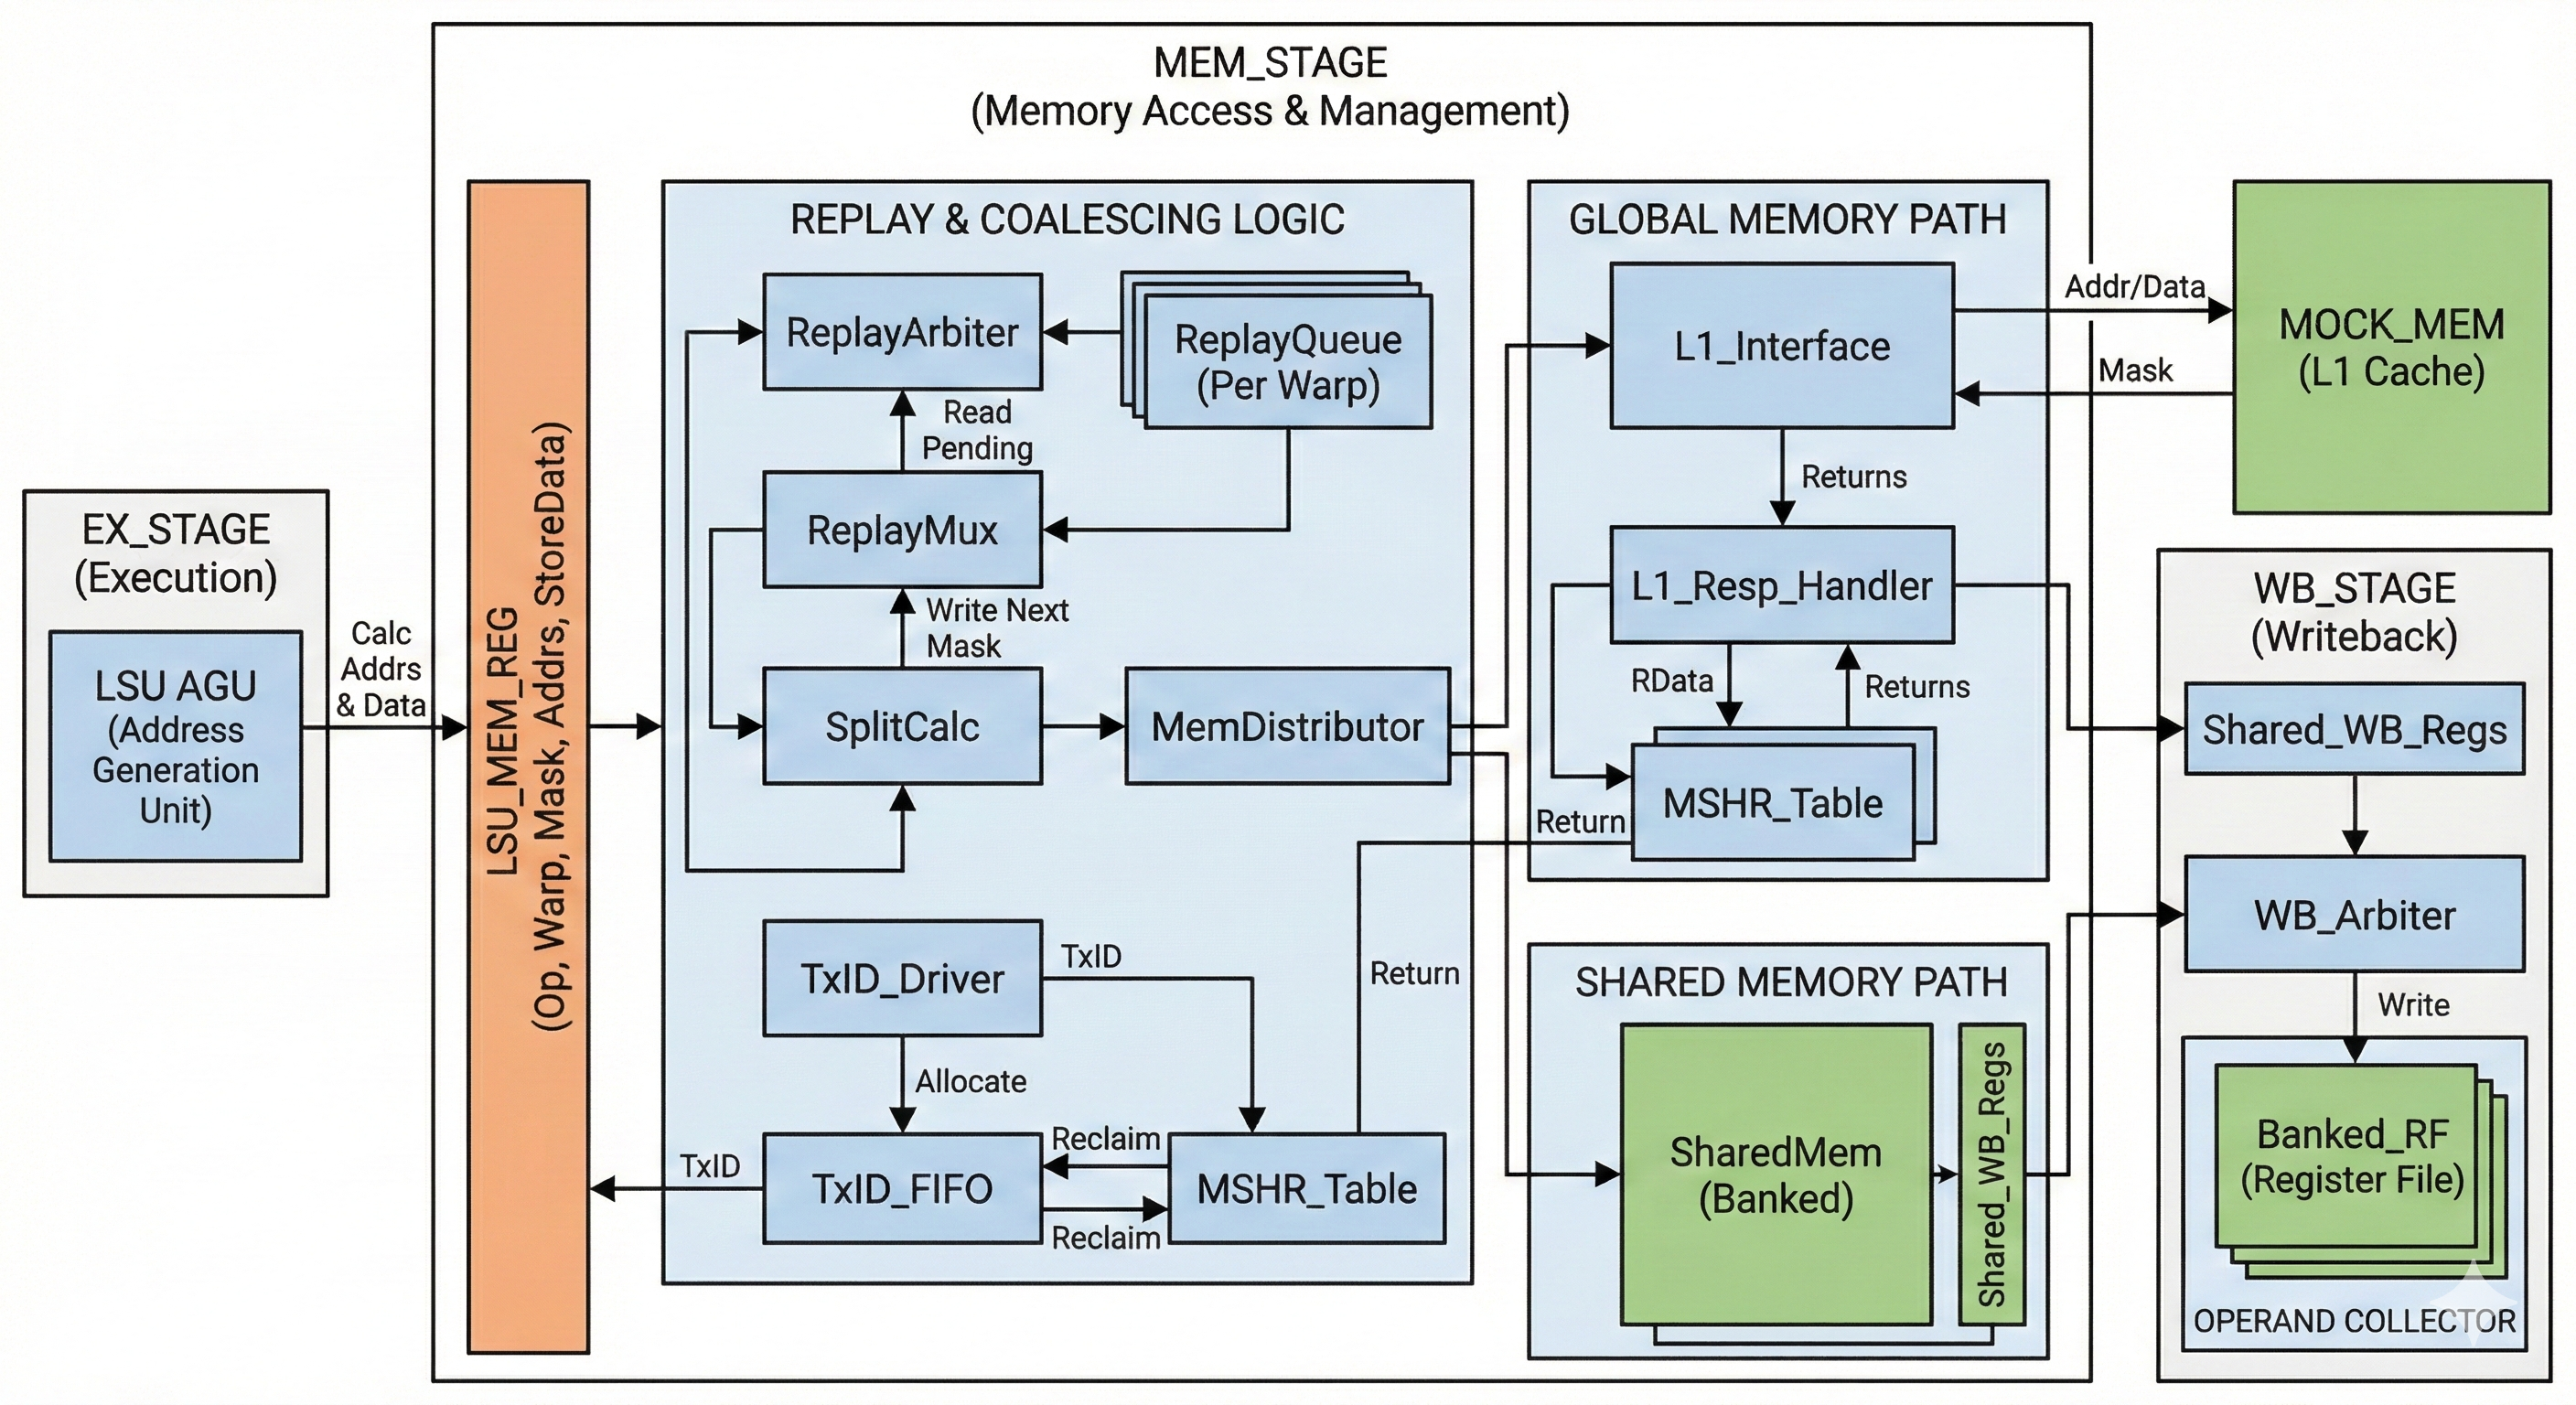
\includegraphics[width=0.9\textwidth]{memory_subsystem.png}
    \caption{LSU and Memory Subsystem Architecture}
    \label{fig:memory}
\end{figure}

\textbf{Data Hazard Prevention}: Even with out-of-order completion, RAW hazards are prevented through the scoreboard. When a load issues, the destination register is immediately scoreboarded. Dependent instructions stall at ID stage until the memory response clears the scoreboard.

\subsection{Barrier Synchronization (Epoch Consistency)}

The hardware barrier (BAR) implements epoch consistency to prevent fast-warp race conditions.

\begin{infobox}{Epoch Mechanism}
\begin{itemize}[leftmargin=*]
    \item \textbf{Problem}: Fast warp could re-enter same barrier before slow warp exits
    \item \textbf{Solution}: Global \texttt{barrier\_epoch} bit toggles on each barrier resolution
    \item \textbf{Guarantee}: Warps only contribute if their local epoch matches global epoch
\end{itemize}
\end{infobox}

Each thread has 7 predicate registers (P0-P6), plus implicit P7 (always true).

\begin{lstlisting}[language=C,caption={Predicate Example}]
ISETP.GT P1, R_x, 0    // Set P1 = (x > 0)
@P1 MUL R_y, R_x, 2    // Only execute if P1 is true
\end{lstlisting}

Execution mask: \texttt{exec\_mask = warp\_active\_mask \& predicate\_mask}

\subsection{3D Graphics Orchestration}

The core features dedicated support for 3D graphics vertex processing. By leveraging the SFU for rotation math and high-throughput integer arithmetic for perspective projection, the SM can orchestrate full 3D wireframe rendering.

\begin{itemize}[leftmargin=*]
    \item \textbf{Perspective Projection}: Hardware-accelerated depth scaling using \texttt{IDIV} for $W$-clipping and perspective divide.
    \item \textbf{Rotation Engine}: High-precision 1.15 fixed-point rotation matrices utilizing the SFU's \texttt{SIN} and \texttt{COS} units.
    \item \textbf{Vertex Shader Pipeline}: Full assembly-level implementation of vertex transformation directly writing to a global framebuffer.
\end{itemize}

\newpage

% ============================================================================
\section{Verification \& Performance}
% ============================================================================

The core includes a comprehensive verification suite focused on GPGPU and Graphics kernels.

\subsection{Benchmark: 8×8 Tiled Matrix Multiplication}

This benchmark verifies $C = A \times B$ for 8×8 matrices using shared memory tiling.

\subsubsection{Why Tiling \& Shared Memory?}

\begin{table}[h]
\centering
\begin{tabular}{|l|l|}
\hline
\textbf{Naive Implementation} & \textbf{Tiled Implementation} \\
\hline
64 global memory accesses/thread & 8 global memory accesses/thread \\
\hline
$\sim$3000+ cycles & 487 cycles \\
\hline
High latency (100-400 cycles) & Low latency (1-2 cycles for shared mem) \\
\hline
\end{tabular}
\caption{Performance Comparison}
\end{table}

\textbf{Benefits}:
\begin{enumerate}[leftmargin=*]
    \item \textbf{Data Reuse}: Load each tile once, reuse across all threads ($\sim$8× reduction in global memory traffic)
    \item \textbf{Low Latency}: Shared memory has $\sim$100× lower latency than global memory
    \item \textbf{Bandwidth Efficiency}: Coalesced loads maximize memory bandwidth utilization
\end{enumerate}

\newpage

\subsection{Performance Metrics}

\begin{table}[h]
\centering
\begin{tabular}{|l|r|}
\hline
\textbf{Metric} & \textbf{Value} \\
\hline
Total Execution Cycles & 487 \\
\hline
Matrix Size & 8×8 \\
\hline
Threads per Warp & 32 \\
\hline
Warps Used & 2 \\
\hline
Shared Memory Usage & 512 bytes \\
\hline
\end{tabular}
\caption{Matrix Multiplication Performance}
\end{table}

\vspace{0.5cm}

\textbf{Verification}: The simulation initializes Matrix A with linear values (1..64) and Matrix B as an Identity matrix. The expected result C is identical to A, which the testbench verifies successfully in 487 cycles.

\vspace{0.5cm}

\begin{verbatim}
Verify: Matrix A (Input)
  [    1    2    3    4    5    6    7    8 ]
  [    9   10   11   12   13   14   15   16 ]
  [   17   18   19   20   21   22   23   24 ]
  [   25   26   27   28   29   30   31   32 ]
  [   33   34   35   36   37   38   39   40 ]
  [   41   42   43   44   45   46   47   48 ]
  [   49   50   51   52   53   54   55   56 ]
  [   57   58   59   60   61   62   63   64 ]

Verify: Matrix B (Input)
  [    1    0    0    0    0    0    0    0 ]
  [    0    1    0    0    0    0    0    0 ]
  [    0    0    1    0    0    0    0    0 ]
  [    0    0    0    1    0    0    0    0 ]
  [    0    0    0    0    1    0    0    0 ]
  [    0    0    0    0    0    1    0    0 ]
  [    0    0    0    0    0    0    1    0 ]
  [    0    0    0    0    0    0    0    1 ]

Verify: Matrix C (Result)
  [    1    2    3    4    5    6    7    8 ]
  [    9   10   11   12   13   14   15   16 ]
  [   17   18   19   20   21   22   23   24 ]
  [   25   26   27   28   29   30   31   32 ]
  [   33   34   35   36   37   38   39   40 ]
  [   41   42   43   44   45   46   47   48 ]
  [   49   50   51   52   53   54   55   56 ]
  [   57   58   59   60   61   62   63   64 ]
=======================================================

TEST PASSED!
Total Cycles: 487
\end{verbatim}

\subsection{Benchmark: 3D Graphics – Perspective Cube}

A dedicated graphics kernel (\texttt{test\_perspective\_cube.sv}) validates the core's ability to orchestrate 3D vertex processing.

\begin{itemize}[leftmargin=*]
    \item \textbf{Shader Logic}: Performs 3D rotations and perspective transformation ($x' = x \cdot f / z$).
    \item \textbf{Hardware Utilization}: Stresses the SFU (trigonometry), IDIV (projection), and the Replay Queue (framebuffer stores).
    \item \textbf{Verification}: Bit-accurate comparison of projected vertex coordinates against a golden Python reference model.
\end{itemize}

\begin{figure}[htbp]
    \centering
    \includegraphics[width=0.6\textwidth]{wireframe_cube.png}
    \caption{3D Wireframe Rendering Output}
    \label{fig:wireframe}
\end{figure}

\subsection{Benchmark: Parallel Vertex Processing}

A parallelized version of the vertex shader (\texttt{test\_parallel\_cube.sv}) was developed to utilize SIMT execution (8 threads).

\begin{table}[h]
\centering
\begin{tabular}{|l|l|l|}
\hline
\textbf{Mode} & \textbf{Total Cycles} & \textbf{Speedup} \\
\hline
Sequential (1 Thread) & 99,312 & 1.0x \\
\hline
Parallel (8 Threads) & 34,368 & \textbf{2.9x} \\
\hline
\end{tabular}
\caption{Vertex Processing Performance}
\end{table}

\noindent \textbf{Analysis}: The parallel implementation achieves a nearly 3x speedup. The theoretical 8x speedup is constrained by the lack of hardware atomic operations, necessitating a serialized framebuffer write loop (software ROP) to prevent race conditions.

\subsection{Regression Suite}

The core is validated against an 11-test regression suite covering all architectural features:

\begin{table}[h]
\centering
\small
\begin{tabular}{|l|p{8cm}|}
\hline
\textbf{Test Name} & \textbf{Feature Validated} \\
\hline
test\_alu\_ops & Basic integer arithmetic and logic \\
\hline
test\_app\_matmul & 8x8 Tiled Matrix Multiplication \\
\hline
test\_control\_flow & Nested branches and divergence stack \\
\hline
test\_fpu\_sfu\_ops & Floating point and transcendental units \\
\hline
test\_function\_call & CALL/RET hardware stack \\
\hline
test\_lsu\_split & LSU memory coalescing and multi-line splits \\
\hline
test\_memory\_system & MSHR and transaction tracking \\
\hline
test\_perspective\_cube & 3D Rendering with Perspective Projection \\
\hline
test\_pipeline\_issue & Dual-issue structural and data hazards \\
\hline
test\_rotated\_cube & Orthographic 3D rotation shader \\
\hline
test\_wireframe\_cube & Basic wireframe rendering demo \\
\hline
\end{tabular}
\caption{SystemVerilog Regression Suite}
\end{table}

\newpage

% ============================================================================
\section{Limitations \& Future Work}
% ============================================================================

\subsection{Current Limitations}

\begin{warnbox}{Rasterization Stage}
The current hardware supports point-based vertex rendering and wireframe logic. Full-triangle rasterization with barycentric interpolation is a future milestone for the dedicated rasterization unit.
\end{warnbox}

\subsection{Future Enhancements}

\begin{itemize}[leftmargin=*]
    \item L1/L2 cache hierarchy integration with genuine set-associative logic
    \item Multi-SM scaling with Network-on-Chip (NoC) interconnect
    \item Hardware Rasterizer and Texture Mapping Unit (TMU) integration
    \item Performance counters and GPGPU profiling support
\end{itemize}

% ============================================================================
\section{Conclusion}
% ============================================================================

The Kepler-Style SIMT Core provides a comprehensive, educational implementation of modern GPU architecture principles. With its dual-issue pipeline, hardware divergence handling, and sophisticated memory subsystem, it serves as an excellent platform for learning GPU microarchitecture and SIMT execution models.

\vspace{1cm}

\begin{center}
\textcolor{xilinxgray}{\rule{0.8\textwidth}{0.4pt}}\\
\vspace{0.5cm}
\textbf{For more information, refer to the RTL implementation in:}\\
\texttt{RTL/Core/streaming\_multiprocessor.sv}
\end{center}

\end{document}
